% !TEX root = ../agglo_clust_review.tex

\begin{figure}
\centering
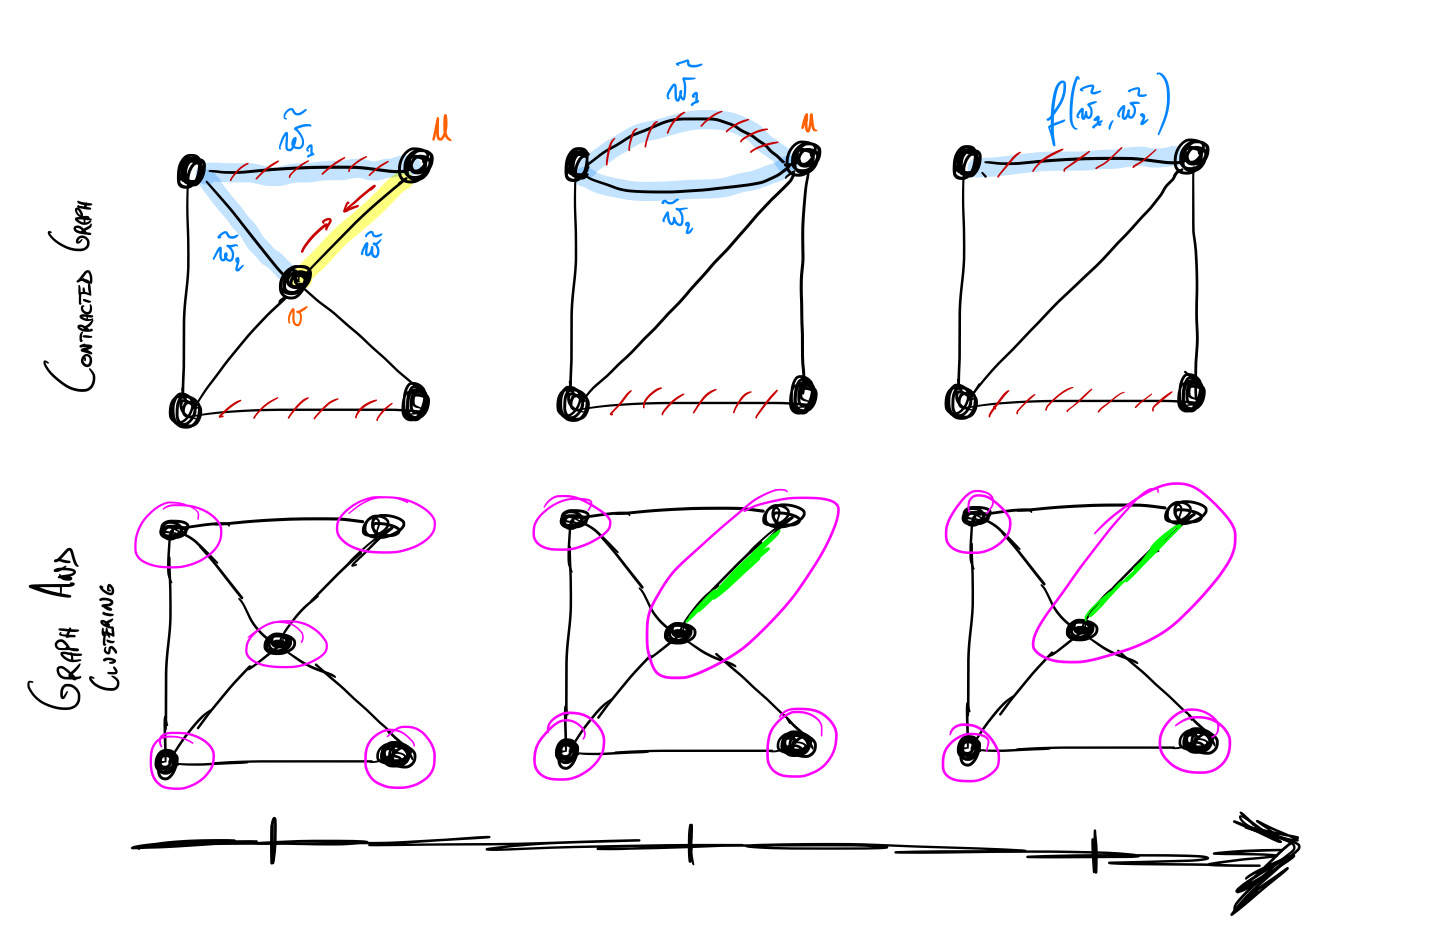
\includegraphics[width=0.50\textwidth,trim=0.in 0.in 0.in 0.in,clip]{./figs/edge_contraction.png}
\caption{\small 
Example of edge contraction: the edge $e_{uv}$ is selected from priority queue; after nodes $u$ and $v$ are merged and $e_{uv}$ is deleted, there are two double edges $e_1$ and $e_2$ left in the graph.  \TODO{Rotate drawings to optimize space}
\label{fig:example_non_unique_weights_1}}
\end{figure}

\begin{algorithm}
  \caption{Unified Graph Agglomerative Clustering}
   \hspace*{\algorithmicindent} \textbf{Inputs:} graph $\mathcal{G}(V,E,W)$; bool {\color{blue}\texttt{addCannotLink}}  \\
  \hspace*{\algorithmicindent} \textbf{Outputs:} Final clustering and contracted graph $\mathcal{G}'$\\
  \hspace*{\algorithmicindent} 
  \begin{algorithmic}[1]


    % \Procedure{SignedGraphEdgeContr}{{\color{blue}bool \emph{addConstraints}}}
      % \State $\mathcal{G}'\gets \mathcal{G}(V,E^+ \cup E^-)$ \Comment{Initialize the contracted graph}
      \State Initialize contracted graph $\mathcal{G}'(V',E')$ from $\mathcal{G}$
      \State Initialize \texttt{canBeMerged}$[e] \gets$ \texttt{True} $\,\,\, \forall e\in E$
      \State Sort edges in priority queue (PQ) in desc. order of $|W_e|$ 
      \State
      \While{PQ is \textbf{not} empty}
        \State Pop edge $e_{uv}\in E'$ with highest abs. priority $|\tilde{w}|$
        \State
        \If{({\color{ForestGreen}\textbf{$\tilde{w} > 0$}}) \textbf{and} \texttt{canBeMerged}$[e_{uv}]$}
          
          % \State PQ, $\,E_\dagger,\,\, E' \gets$ \textsc{deleteDoubleEdges}($u,v$)
          
        %   \State Update costs of double edges;
        %   \State Propagate constrained flags of double edges;
          \State Contract $e_{uv}$ in $\mathcal{G}'$
          \For{every new pair of double edges $(e_1,e_2)$}
            \State Get priorities $\tilde{w}_1, \tilde{w}_2$ of $e_1,e_2$
            \State Use update rule $f(\tilde{w}_1,\tilde{w}_2)$ (see Table 1) to 
            \Statex \hspace{\algorithmicindent}\hspace{\algorithmicindent}\hspace{\algorithmicindent}\hspace{\algorithmicindent} update priority of $e_1$
            \State Delete $e_2$ from $\mathcal{G}'$
          \EndFor
          % \State  Replace double edges in $\mathcal{G}'$ with single edges
          % \Statex \hspace{\algorithmicindent}\hspace{\algorithmicindent}\hspace{\algorithmicindent} and update priorities
        \EndIf
        \State
        \If{({\color{red}\textbf{$\tilde{w} \leq 0$}}) \textbf{and} {\color{blue}\texttt{addCannotLink}}}
          % \State Flag $e_{uv}$ as MustNotLink
          \State \texttt{canBeMerged}$[e_{uv}] \gets$ \texttt{False}
        \EndIf
      \EndWhile


      % \For{$e  \in E$ in descending order of absolute costs $|W(e)|$}
      %   \If{({\color{ForestGreen}\textbf{$W(e) > 0$}}) \textbf{AND} (edge is not constrained)}
      %     \State Contract edge $e$ in the graph $\mathcal{G}'$;
      %     \State Update costs of double edges;
      %     \State Propagate constrained flags of double edges;
      %     % \For{every new double edge}
      %     %   \State Delete double edges
      %     %   \State Insert new one with updated cost
      %     % \EndFor
      %   \EndIf
      %   \If{({\color{red}\textbf{$W(e) \leq 0$}}) \textbf{AND} ({\color{blue}\emph{addConstraints}})}
      %     \State Flag edge $e$ as constrained
      %   \EndIf
      % \EndFor
      \State
      \State
      \Return $\mathcal{G}'$
      % \State


    % \EndProcedure

  \end{algorithmic}
  \label{main_alg}
\end{algorithm}


\begin{figure}
\centering
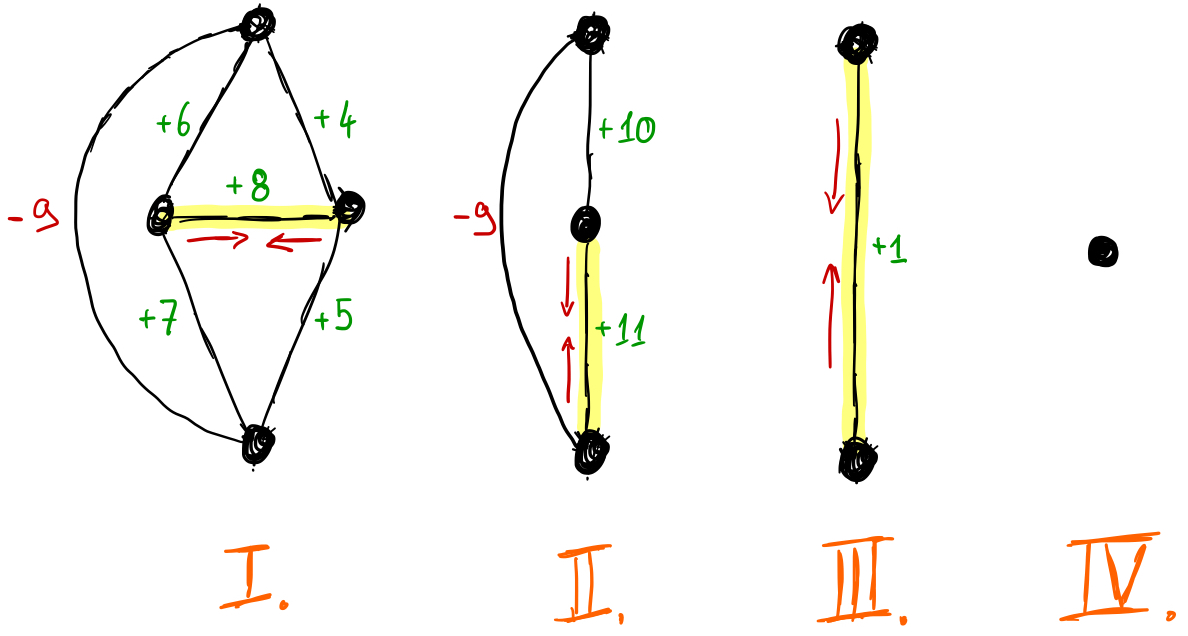
\includegraphics[width=0.45\textwidth,trim=0.in 0.in 0.in 0.in,clip]{./figs/aggl_clust.png}
\caption{\small 
Example of agglomerative clustering on signed graph with sum update rule and without Cannot-Link-Constraints. The final clustering is given by one single cluster.
\label{fig:example_non_unique_weights_1}}
\end{figure}


\begin{figure}
\centering
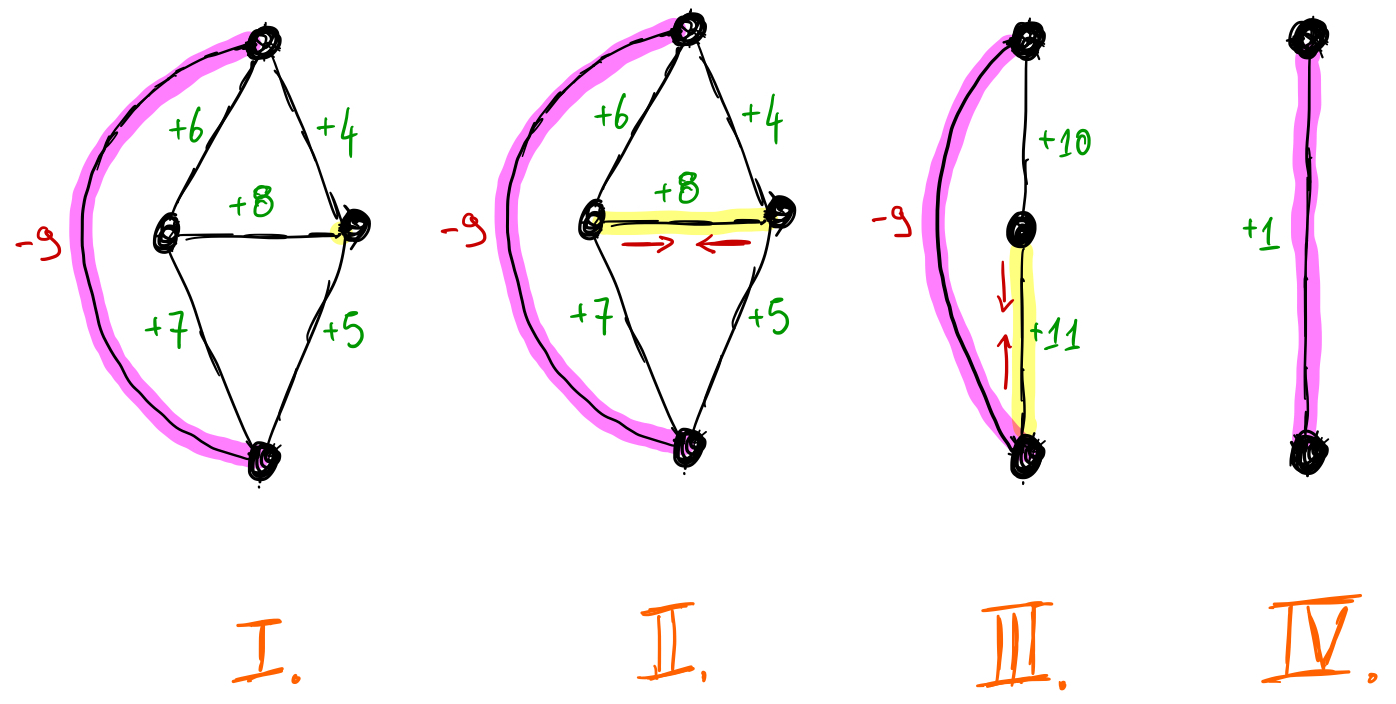
\includegraphics[width=0.50\textwidth,trim=0.in 0.in 0.in 0.in,clip]{./figs/aggl_clust_with_nonlink.png}
\caption{\small 
Example of agglomerative clustering on signed graph with sum update rule and using Cannot-Link-Constraints. Edges flagged with \texttt{canBeMerged} = \texttt{False} are highlighted in pink. 
\label{fig:example_non_unique_weights_2}}
\end{figure}


\begin{table*}[h]
    \centering
    \begin{subtable}[t!]{0.98\textwidth}\centering
        \begin{tabular}{r l || c | c | c}
            % \toprule\toprule
             & &  \multirow{3}{*}{\textbf{Unsigned graphs}}  & \multicolumn{2}{c}{\textbf{Signed graphs}}  \\        
            % \cmidrule(l{.15em}){4-5}
            % \cline{4-5}
            & & &  \multicolumn{2}{c}{\thead{Use Cannot-Link-Constraints:}} \\        
           
            & & &  \thead{NO} & \thead{YES} \\        
            % \cmidrule[0.3em]{3-5}
            % \midrule[0.15em]
            \midrule\midrule
            Sum: & $f(\tilde{w}_1,\tilde{w}_2) = \tilde{w}_1+\tilde{w}_2$ & \thead{Sum Linkage\\Hierarchical Clustering} & \thead{Greedy Additive \\ Edge Contraction \cite{levinkov2017comparative}} & \thead{Greedy Fixation \cite{levinkov2017comparative}} \\ \midrule
            
            \makecell[r]{Absolute \\ maximum:} & \makecell[l]{$f(\tilde{w}_1,\tilde{w}_2) =\argmax_{\tilde{w}\in\{\tilde{w}_{1},\tilde{w}_{2}\}} \big|\tilde{w} \big| $}   & \thead{Single Linkage\\Hierarchical Clustering\\ \cite{lance1967general}} & \thead{Mutex Watershed \cite{wolf2018mutex}} & \thead{Mutex Watershed \cite{wolf2018mutex}} \\ \midrule

            \makecell[r]{Arithmetic \\mean:} & $f(\tilde{w}_1,\tilde{w}_2) = \mathrm{weightedAvg}\{ \tilde{w}_1, \tilde{w}_2 \} $                                 & \thead{ Average Linkage\\ Hierarchical Clustering \\(UPGMA) \cite{lance1967general}} & \thead{Signed Agglomerative Clust. \\ with Average Linkage \\ (\textbf{NEW})} & \thead{\textbf{NEW}}\\ \midrule

            Maximum: & $f(\tilde{w}_1,\tilde{w}_2) = \max \{ \tilde{w}_1, \tilde{w}_2 \}  $                                 & \thead{Single Linkage\\Hierarchical Clustering\\ \cite{lance1967general}} & \thead{Signed Agglomerative Clust. \\ with Single Linkage \\ (\textbf{NEW})} & \thead{\textbf{NEW}}\\ \midrule

            Minimum:& $f(\tilde{w}_1,\tilde{w}_2) = \min \{ \tilde{w}_1, \tilde{w}_2 \}  $                                 & \thead{Complete Linkage\\ Hierarchical Clustering \\ \cite{lance1967general}}  & \thead{Signed Agglomerative Clust. \\ with Complete Linkage \\ (\textbf{NEW})} & \thead{\textbf{NEW}}



            
        \end{tabular}
        % \caption{Linkage criteria}
    \end{subtable} 
    \caption{The table lists all the algorithms that can be seen as special cases of the Generic Agglomerative Clustering \ref{main_alg} given a specific update rule $f(e_1,e_2)$ and a type of graph...}
    \label{tab:linkage-criteria}
\end{table*}



\section{Unified Graph Agglomerative Clustering \\Algorithm}
In this section we introduce a unified agglomerative clustering algorithm that represents a simple generalized formalization of many agglomerative graph clustering algorithms. It can be used to describe both unsigned clustering algorithms ingesting positive similarities between clusters and signed clustering algorithms using attractive and repulsive cues.\\
First, we define the graph notation and the concept of cannot-link constraints. Then, we introduce the generalized algorithm and show \UPDATE{how it can be used to introduce several new agglomerative clustering algorithms for graphs with signed weights.}

\subsection{Graph notation and cannot-link constraints}

\begin{itemize}
\item Define graph formalism and clustering $\Pi$. Make comment about special case of unsigned graph!
\item Introduce concept of cannot-link-constraints
\item From wiki: \emph{Both a must-link and a cannot-link constraint define a relationship between two data instances. A must-link constraint is used to specify that the two instances in the must-link relation should be associated with the same cluster. A cannot-link constraint is used to specify that the two instances in the cannot-link relation should not be associated with the same cluster. These sets of constraints acts as a guide for which a constrained clustering algorithm will attempt to find clusters in a data set which satisfy the specified must-link and cannot-link constraints. Some constrained clustering algorithms will abort if no such clustering exists which satisfies the specified constraints. Others will try to minimize the amount of constraint violation should it be impossible to find a clustering which satisfies the constraints.}

\end{itemize}
\subsection{The algorithm}
\begin{itemize}
\item First give intuitive idea of agglomerative clustering
\item enforce the fact that the cannot-link relations are introduced \textbf{dynamically}

\item \textbf{Specific description:} The algorithm proceeds as follows: it initializes a contracted graph $\mathcal{G}'$ from the original graph $\mathcal{G}$ and it sorts the edges $e\in E$ in a priority queue (PQ) in descending order of absolute value  of the weight, so that the most attractive and the most repulsive edges are analyzed first. The algorithm has two variants: the first one a

At each iteration, one edge is popped from PQ and it is processed only if it belongs to the contracted graph $\mathcal{G}'$. The algorithm terminates when all edges have been processed. and it has two variants: one adding cannot link constraints and one not using them.
\item Comment about must-not-link relations: they give high priority to the most confident repulsive edges 
% \item I don't think I need to mention the merge tree (although it could be easily deduced from the code, as a sequence of clustering)
\item comment about complexity (depends on the linkage criteria) and how dense is the graph (check PQ update)

\end{itemize}

\subsection{Update rules and associated algorithms}
\begin{itemize}
\item Linkage criteria in the table:
\begin{itemize}
\item Mutex Watershed \cite{wolf2018mutex}, [proof of equivalence included in Appendix, also showing that adding or not CLC does not change anything]
\item Greedy Additive Edge Contraction \cite{levinkov2017comparative}, 
\item Greedy Fixation \cite{levinkov2017comparative}, 
\item Hierarchical Agglomerative Clustering with single, complete, average (UPGMA) linkage criteria
\end{itemize}
\item comment about the fact that sum is not an ultra-metric (say better)
\item In this article we analyze only the simplest (and cheapest) types of update rules, but... Easily generalizable for: learned linkage criteria \cite{nunez2013machine}, something depending on node size \cite{felzenszwalb2004efficient}, quantiles, weighted average (WPGMA) and weighted sum (and related work by Paul)


% \begin{table*}[t]
%     \centering
%     \begin{subtable}[t!]{0.98\textwidth}\centering
%         \begin{tabular}{c | c }
%             \toprule\toprule
%             \makecell{Algorithm name} & \makecell{Algorithm description and \\linkage criteria}    \\
%             \midrule\midrule

%             Weighted Arithmetic Mean (WPGMA) & \thead{Assign a weighting $\alpha_e \in \mathbb{R}^+$, $\forall e \in E$ \\ \\ Linkage criteria: $w_{\mathrm{new}} = \frac{\alpha_1 w_1 +\alpha_2 w_2}{\alpha_1 + \alpha_2} $}  \\ \midrule
            
%             \makecell{Felzenszwalb Efficient \\Graph-based Image Segmentation \cite{felzenszwalb2004efficient}}  & \thead{Initially all edges have positive weights }  \\ \midrule

%             \makecell{Quantile Agglomeration Clustering (...?)}  & \thead{...}  \\ \midrule

%             \makecell{Graph-based active learning \\of agglomeration (GALA) \cite{nunez2013machine}}  & \thead{Assign set of edge features $\phi^{\mathrm{I}}_e$ and \\node features $\phi^{\mathrm{II}}_u$, $\forall u \in V$, $\forall e \in E$. \\ \\ A classifier $f$ with parameters $\theta$ predicts and updates\\ the cost of an edge: $w_e = f(\phi^{\mathrm{I}}_e, \phi^{\mathrm{II}}_u, \phi^{\mathrm{II}}_v; \theta)$, $\forall e_{uv} \in E$} \\ \midrule

%             % \makecell{$w_{\mathrm{new}}=w_{\tilde{e}}$,$\,
%             % \,$ where $\tilde{e}=\mathrm{arg}\max_{e\in \{e_{1},e_{2}\}} \left|w_e\right|$  }  & \thead{Mutex Watershed \cite{wolf2018mutex}} & \thead{Mutex Watershed \cite{wolf2018mutex}} \\ \midrule

%             % Arithmetic mean: $w_{\mathrm{new}} = (w_1+w_2) / 2 $                                 & \thead{Hierarchical Clustering \\ with Average Linkage (UPGMA)} & \thead{\textbf{NEW}}\\ \midrule

%             % Maximum: $w_{\mathrm{new}} = \max \{ w_1, w_2 \}  $                                 & \thead{Hierarchical Clustering \\ with Single Linkage} & \thead{\textbf{NEW}}\\ \midrule

%             % Minimum: $w_{\mathrm{new}} = \min \{ w_1, w_2 \}  $                                 & \thead{Hierarchical Clustering \\ with Complete Linkage} & \thead{\textbf{NEW}}



            
%         \end{tabular}
%         % \caption{Linkage criteria}
%         \label{tab:linkage-criteria}
%     \end{subtable} 
%     \caption{Linkage criteria 2}
% \end{table*}



\end{itemize}
